% ADD/REMOVE THE 'answers' OPTION TO INCLUDE/SUPPRESS SOLUTIONS
% \documentclass[11pt,addpoints]{exam}
\documentclass[11pt,addpoints, answers]{exam}

\newcommand{\hwnum}{8}
\newcommand{\duedate}{March 26}

% In order to compile this file you will need to get 'header.tex'
% and make the line below point to the appropriate file path
\input{header}
\usepackage{array}
\usepackage{multicol}

\newcommand{\ptimemap}{\leq_p}
\newcommand{\tred}{\leq_T}
\newcommand{\ans}[1]{\ifprintanswers{\textcolor{blue}{#1}} \else  \fi}

\ifprintanswers
\hwslnheader   % header for solutions
\else
\hwheader   % header for homework
\fi

\begin{document}

\begin{questions}

  \question[10] \textbf{Self assessment.} \nopagebreak
  
  Carefully read and understand the posted solutions to the previous homework.
  Identify one part for which your own solution has the most room for improvement (e.g., has unsound reasoning, doesn’t show what was required, could be significantly clearer or better organized, etc.).
  Copy or screenshot this solution, then in a few sentences, explain what was deficient and how it could be fixed.

  (Alternatively, if you think one of your solutions is significantly \emph{better} than the posted one, copy it here and explain why you think it is better.)

  If you didn't do last week's homework, choose a problem from it that looks challenging to you, and in a few sentences, explain the key ideas behind its solution in your own words.

  \begin{solution} 
  My answer for question 4 (a) was as follows:

  \begin{solution} 
  Suppose there is a polynomial-time mapping reduction from \(A\) to \(B\) via a function \(f\). On input \(x\):
  \begin{enumerate}
      \item Compute \(f(x)\) in polynomial time.
      \item Query the oracle for \(B\) on \(f(x)\).
      \item Accept if the oracle says ``yes,'' and reject otherwise.
  \end{enumerate}
  This is a Turing reduction from \(A\) to \(B\), so \(A \tred B\).
  \end{solution}

  This turing reduction is correct, but I forgot to include a correctness proof. This correctness proof would show that if \(x \in A\), then \(f(x) \in B\), and if \(x \notin A\), then \(f(x) \notin B\). Otherwise, my homework 7 had no other big issues.
  
  \end{solution}

  \pagebreak
  \question \textbf{True, false, or unknown.}
  
    For each of the following statements, state, with brief justification, that it is \emph{known to be true}, \emph{known to be false}, or its truth/falsehood is \emph{unknown}. If the statement is known to be false, either give a counterexample or briefly explain which part of the statement is false. 

    \begin{parts}
        \part [4] If $\P \neq \NP$ and $L$ is $\NP$-complete, then $L \notin \P$.

        \begin{solution}  
        Known to be true; placing an NP-complete language in \(\P\) implies \(\P = \NP\).  
        \end{solution} 

        \part [4] If $L\in\NP$, then $L \in \P$.

        \begin{solution}  
        Unknown; whether \(\P = \NP\) or not remains an open question.  
        \end{solution}  

        \part [4] Let $V$ be an efficient verifier for some language $L \in \NP$. Let $f$ be the Cook-Levin mapping reduction from $L$ to $\SAT$. The function $f(x)$ selects a certificate $c$, runs $V(x,c)$, and construct a Boolean formula $\phi$ from its computational tableau. 

        \begin{solution}  
        Known to be false; the reduction cannot choose a specific certificate \(c\) because it only has access to the input \(x\), not any valid witness.
        \end{solution}
        
    \end{parts}

  
  \pagebreak
  \question \textbf{$\Upsilon$'s alternative reductions.}

  Professor $\Upsilon$ is impressed by the polynomial-time mapping reductions presented in the past few lectures. However, $\Upsilon$ thinks some of them have alternative solutions and presents to you here. 

  For each of the following reduction, identify the flaw(s) in the reduction and briefly explain why it fails. You may support your answers with counterexamples. 

  \begin{parts}
      \part [5] In lecture, we proved that $\HC \ptimemap \TSP$, where
  \begin{align*}
    \HC &= \set{ G : G \text{ is an unweighted graph with a Hamiltonian cycle}} \\
    \TSP &= \set{ (G, k) : G \text{ is a weighted, complete graph with a tour of weight} \leq k }
           \; \text.
  \end{align*}
  
  $\Upsilon$ notices that $\HC$ is itself decidable. They attempt to first find a Hamiltonian cycle in the graph and then set the weights of the edges in that cycle to $1$, while assigning a weight of $\infty$ to all other edges. This ensures that the TSP instance has a tour of weight at most $|V|$ iff the original graph contains a Hamiltonian cycle.
      
      \begin{minipage}{0.9\textwidth}
      \begin{center}
    \begin{algorithm}[H]
      \begin{algorithmic}[1]
      \Require{An unweighted graph $G$}
      \Ensure{A weighted graph $G'$ and nonnegative integer $k$}
        \Function{$f$}{$G=(V,E)$}
        \State $V' \gets V$
        \State Initialize $G'$ to be a complete graph on $V'$ and initialize all weights to $\infty$ in $E'$
        \State Initialize $C$ to be an empty sequence of vertices
        \For{each permutation $\Pi = (v_1, v_2, \ldots, v_n)$ of $V$}
            \If {$(v_i, v_{i+1}) \in E$ for all $i = 1, \ldots, n-1$} 
                \State $C \gets \Pi$
                \State \textbf{break}
            \EndIf
        \EndFor
        \For {each adjacent pair $(v_i, v_{i+1})$ in $C$}
            \State Set the weight of $(v_i, v_{i+1})$ to be 1 in $E'$
        \EndFor
        \State \Return $(G'=(V', E'), k=\abs{V})$
        \EndFunction
      \end{algorithmic}
    \end{algorithm}
    \end{center}
    \end{minipage}


    \begin{solution} 
    \begin{itemize} 
      \item The construction attempts to locate a Hamiltonian cycle in \(G\) by enumerating permutations, which solves \HC{} directly and is not known to run in polynomial time. A valid polynomial-time reduction cannot depend on having a solution to \HC{} in order to build the new instance.
      \item If no Hamiltonian cycle is found, all edges receive weight \(\infty\), producing no valid TSP tour. This incorrectly discards the possibility of constructing a valid polynomial-time instance when the original graph has no Hamiltonian cycle, and thus fails as a reduction. 
    \end{itemize} 
    \end{solution}

      \part [5] In lecture, we also proved that $\TSAT \ptimemap \VC$, where
      \begin{align*}
          \TSAT &= \set{\phi: \text{$\phi$ is a satisfiable 3CNF formula}} \\
          \VC &= \set{(G,k): \text{$G$ is a graph with a vertex cover of size (at most) $k$}}.
      \end{align*}
      
      $\Upsilon$ thinks the reduction can be simplified. They propose that each variable ``gadget'' \emph{should not have an edge between its two vertices}. Everything else about the reduction is left unchanged, i.e., 

      \begin{itemize}
          \item For each variable $x \in \phi$, create a variable gadget
           consisting of two vertices, respectively labeled by the literals $x$ and $\overline x$, with \emph{no edges between them}. 
           \item For each clause $(\ell_i \lor \ell_j \lor \ell_k)$ in $\phi$, create a clause gadget of three vertices, respectively labeled by these literals, with an edge between each pair of these vertices (i.e., a triangle).
           \item For each vertex of each clause gadget, create an edge between that vertex and the (unique) variable-gadget vertex having the same label. 
           \item Finally, set $k = n+2m$, where $n$, $m$ are respectively the number of variables and clauses in $\phi$. 
      \end{itemize}

      \begin{solution} 
      Without an edge between each pair of variable-literal vertices, the construction no longer enforces having exactly one literal per variable. Both or neither literals can appear in the vertex cover, invalidating the intended one-to-one correspondence between vertex cover and truth assignment.
      \end{solution}
      
  \end{parts}

    \question \textbf{Scheduling exams with flying colors.} 

\newcommand{\Coloring}
{\textsc{Coloring}}
\newcommand{\Schedule}{\textsc{Scheduling}}

    The EECS 376 staff email has been flooded with complaints about exam conflicts. To resolve this, they plan on working with the registrar's office to determine whether or not the exams can be scheduled so that no student has an exam conflict with another class. 

    As 376 staff, they have defined the problem as a language. Given a set of students $S$, a collection of subsets $C = \set{C_1, \ldots, C_n}$ of $S$ where each $C_i$ represents the students enrolled in course $i$, and the number of exam slots $k$, they want to know if each course can be assigned to an exam slot such that no student has two exams in the same slot. 

    Formally, the language $\Schedule$ is defined as follows:  
    \[
        \Schedule = \set{(S, C, k): \exists f: C \rightarrow \{1 \ldots k\} \text{ s.t } f(C_i) = f(C_j) \implies C_i \cap C_j = \emptyset}
    \]
    As a star student in EECS 376, you recognize a potential challenge. The problem the staff has defined resembles a well-known computationally difficult problem. Save the day by proving that $\Schedule$ is NP-hard!


        \begin{parts}
            \part [6] You recall from the end of L17 that the Coloring Problem is NP-complete.\footnote{If interested, \href{https://www.geeksforgeeks.org/3-coloring-is-np-complete/}{here}'s the \NP-completeness proof for the $3\textsc{-Coloring}$ problem. With a little more work, it can be generalized to $\Coloring$. You do not need to know the proof for this class, all you need is that $3\textsc{-Coloring}$ and $\Coloring$ are \NP-complete.} A graph is colorable by $k$ colors if the vertices can be colored such that for any given edge $(u,v)$, $u$ and $v$ have different colors. Formally, we can define it as follows: 
        \[
        \Coloring = \{ (G, k): G\text{ is colorable by }k \text{ colors}    \}.
        \]
        Determine if each of the following is an instance of $\Coloring$. If $(G,k) \in \Coloring$, give a coloring of the graph.\footnote{You may give the vertex-color pairs, a table, etc. If you want to color the given graph in \LaTeX, you can change the color of a node using \texttt{\textbackslash node[fill=<color>].}} Otherwise, briefly explain why it's not possible.

    \begin{enumerate}[(i)]
        \item $G = $
            \begin{minipage}{0.3\linewidth}
            \centering
    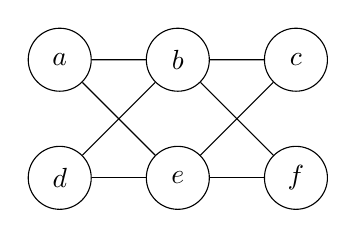
\begin{tikzpicture}[scale=1.5, every node/.style={draw, circle, minimum size=0.8cm, inner sep=0pt}]
        % Define the nodes
        \node (A) at (0,1) {$a$};
        \node (B) at (1,1) {$b$};
        \node (C) at (2,1) {$c$};
        \node (D) at (0,0) {$d$};
        \node (E) at (1,0) {$e$};
        \node (F) at (2,0) {$f$};
    
        \begin{scope}[every node/.style={auto, draw=none}]
        \draw (A) -- (B);
        \draw (A) -- (E);
        \draw (B) -- (C);
        \draw (B) -- (D);
        \draw (B) -- (F);
        \draw (C) -- (E);
        \draw (D) -- (E);
        \draw (E) -- (F);
        \end{scope}
    \end{tikzpicture}
            \end{minipage}
            , $k = 3$

            \begin{solution}
            \[
            a \mapsto 1,\quad b \mapsto 2,\quad c \mapsto 3,\quad d \mapsto 1,\quad e \mapsto 2,\quad f \mapsto 3.
            \]

            \begin{center}
              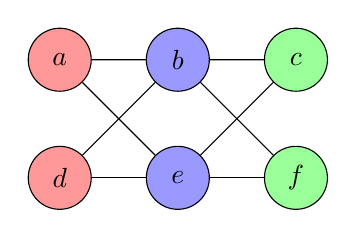
\begin{tikzpicture}[scale=1.5, every node/.style={draw, circle, minimum size=0.8cm, inner sep=0pt}]
                  % Define the nodes with assigned colors
                  \node[fill=red!40] (A) at (0,1) {$a$};    % Color 1
                  \node[fill=blue!40] (B) at (1,1) {$b$};   % Color 2
                  \node[fill=green!40] (C) at (2,1) {$c$};  % Color 3
                  \node[fill=red!40] (D) at (0,0) {$d$};    % Color 1
                  \node[fill=blue!40] (E) at (1,0) {$e$};   % Color 2
                  \node[fill=green!40] (F) at (2,0) {$f$};  % Color 3
              
                  % Draw the edges
                  \begin{scope}[every node/.style={auto, draw=none}]
                  \draw (A) -- (B);
                  \draw (A) -- (E);
                  \draw (B) -- (C);
                  \draw (B) -- (D);
                  \draw (B) -- (F);
                  \draw (C) -- (E);
                  \draw (D) -- (E);
                  \draw (E) -- (F);
                  \end{scope}
              \end{tikzpicture}
            \end{center}
            \end{solution}
            
            \item $G = $
            \begin{minipage}{0.3\linewidth}
            \centering
    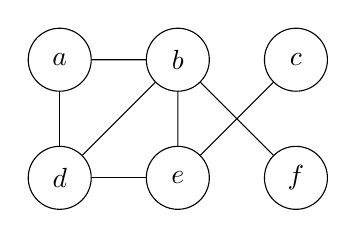
\begin{tikzpicture}[scale=1.5, every node/.style={draw, circle, minimum size=0.8cm, inner sep=0pt}]
        % Define the nodes
        \node (A) at (0,1) {$a$};
        \node (B) at (1,1) {$b$};
        \node (C) at (2,1) {$c$};
        \node (D) at (0,0) {$d$};
        \node (E) at (1,0) {$e$};
        \node (F) at (2,0) {$f$};
    
        \begin{scope}[every node/.style={auto, draw=none}]
        \draw (A) -- (B);
        \draw (A) -- (D);
        \draw (B) -- (D);
        \draw (B) -- (E);
        \draw (B) -- (F);
        \draw (C) -- (E);
        \draw (D) -- (E);
        \end{scope}
    
    \end{tikzpicture}
    \end{minipage}
    , $k = 2$

    \begin{solution}
    Not possible to 2-color, because there is an odd cycle \((a,b,d)\).
    \end{solution}
    \end{enumerate}

            \part [12] Show that $\Coloring \ptimemap \Schedule$. Since $\Coloring$ is \NP-hard, $\Schedule$ is \NP-hard.

        \begin{solution} 
        Given \((G,k)\) from \(\Coloring\) with \(G=(V,E)\), construct 
        \[
        S \;=\; E,\quad C \;=\; \{\,C_v \mid v \in V\},
        \]
        and assign each course \(C_v\subseteq S\) by placing every edge in \(E\) incident to \(v\) into \(C_v\). If $k$ is the number of exam slots, define \(f(G,k)=(S,C,k)\).

        \begin{itemize}
        \item (\(\Rightarrow\)) If \(G\) is colorable by \(k\) colors, color each vertex \(v\) by a color in \(\{1,\dots,k\}\), with a course slot for each color. Assign course \(C_v\) to the slot of the color of \(v\). No adjacent vertices share a color, so no two courses sharing a student occupy the same slot.
        \item (\(\Leftarrow\)) If there is a valid assignment of courses to \(k\) slots, then no two courses sharing a student are placed in the same slot. Thus, no two adjacent vertices share a color in \(G\). This yields a proper \(k\)-coloring.
        \end{itemize}
        Thus \(\Coloring \ptimemap \Schedule\), implying \(\Schedule\) is \NP-hard.

        Constructing \(S\) and \(C\) requires only a single pass through \(V\) and \(E\), so \(f\) runs in polynomial time.
        \end{solution}
        \end{parts}
      
    \pagebreak


    \newcommand{\Clique}
    {\textsc{Clique}}
    \newcommand{\Recipe}
    {\textsc{Bussin-Recipe}}
    
    \question [12] \textbf{This recipe is bussin but \NP-hard.} 
    
    We want to become a famous chef by creating a new dish.  There are $n$ ingredients, and we wish to use $m$ of them ($m\leq n$) of them to create a new dish.  There is an $n \times n$ matrix~$D$ that indicates the \emph{discord} between two ingredients.  In this case, each entry $D_{ij}$ of the matrix~$D$ is an integer value between 0 and 10 (inclusive), where 0 means that the items $i$ and $j$ go together perfectly (there is no discord) and a 10 means they go together very badly.  Any dish prepared with these ingredients is charged the sum of all pairs of ingredients as a penalty. If we can create a dish using at least $m$ ingredients with a total penalty of at most $p$, the recipe is \emph{bussin}.

    Formally, this can be defined as:
    \[
        \Recipe = \set{(D, m, p) : D \in \set{0 \ldots 10}^{n \times n} \text{, } \exists S \subseteq \{1 \ldots n\} \text{ s.t } |S| \geq m \text{ and } \sum_{i,j \in S} D_{ij} \leq p}
    \]
    We assume for simplicity that $D_{ij} = D_{ji}$ and $D_{ii} = 0$ for all $i,j = 1, \ldots n$. 
    
Show that \Recipe\xspace is \NP-hard.

\begin{solution}
Given an instance \((G,k)\) of \Clique\ with \(G=(V,E)\) and \(|V| = n\), construct \(\bigl(D,m,p\bigr)\) as follows:
\[
m \;=\; k,\quad p \;=\; 0,\quad 
D_{ij} \;=\;
\begin{cases}
0 & \text{if } i=j \text{ or } (i,j)\in E,\\
10 & \text{otherwise}.
\end{cases}
\]
\begin{itemize}
\item (\(\Rightarrow\)) If \(G\) has a clique of size \(k\), then there is a set \(S\subseteq\{1,\dots,n\}\) with \(|S|\ge m\) and total penalty \(\sum_{i,j \in S}D_{ij}=0\le p\). 
\item (\(\Leftarrow\)) If there is a set \(S\) with \(|S|\ge m\) and \(\sum_{i,j\in S}D_{ij}\le p\), then all pairs \((i,j)\in S\) must satisfy \(D_{ij}=0\), implying \((i,j)\in E\). Hence \(S\) is a clique of size \(k\). 
\end{itemize}
Thus \(\Clique \le_p \Recipe\), and \(\Recipe\) is \NP-hard.

Building the matrix \(D\) requires checking each pair \((i,j)\) in \(E\); this is achievable in polynomial time.
\end{solution}
  

  \question \textbf{Subset sum.} \nopagebreak

  Recall that a multiset is just like a set, but can have duplicate elements.
  A submultiset also can have duplicate elements, as long as it does not have more copies of any specific element than its containing set does.\footnote{With a little more work, the version with ordinary sets can also be proved $\NP$-complete.}

  Define the language
  \[ \SSUM = \set{(A, s) : A \text{ is a multiset of integers $\geq 0$, and } \exists\; I \subseteq A \text{ s.t } \sum_{a \in I} a = s}.
  \]
  In this problem you will prove that $\TSAT \leq_p \SSUM$, thereby showing that $\SSUM$ is $\NP$-hard.
  Because $\SSUM \in\NP$ (from HW 7), this implies that $\SSUM$ is $\NP$-complete.

  The reduction is as follows.
  As input it is given a 3CNF formula~$\phi$ with~$n$ variables $x_1, \ldots, x_n$ and~$m$ clauses $c_1, \ldots, c_m$.
  (Recall that each clause is the OR of exactly three literals, where a literal is either some variable~$x_{i}$ or its negation $\overline{x_{i}}$.)

  The reduction constructs a collection of numbers as follows:

  \begin{enumerate}
  \item For each clause $c_j$, it constructs integers $a_j=b_j$, which are $m + n$ decimal digits long (counting any leading zeros), whose $j$th digits are~1, and whose other digits are~0.
  \item For each variable $x_i$, it constructs integers $t_i$ and $f_i$, each $m + n$ decimal digits long, where:
    \begin{enumerate}
    \item The $(m + i)$th digits of both $t_i$ and $f_i$ are 1.
    \item The $j$th digit of $t_i$ is 1 if literal $x_i$ appears
      in clause $c_j$.
    \item The $j$th digit of $f_i$ is 1 if literal $\overline{x_i}$
      appears in clause $c_j$.
    \item All other digits of $t_i$ and $f_i$ are 0.
    \end{enumerate}
  \item It constructs a target sum~$s$ that has $m + n$ decimal digits, where the first~$m$ digits are~\textbf{[TODO: \cref{ss-step3}]} and the last~$n$ digits are~\textbf{[TODO: \cref{ss-step3}]}. 
  \end{enumerate}
  The reduction outputs $(A,s)$, where $A$ is the set of all the numbers $a_{j}$, $b_{j}$, $t_{i}$, and~$f_{i}$.

  For example, for the formula $\phi = (x_1 \vee \overline{x_2} \vee x_3) \wedge (\overline{x_1} \vee x_2 \vee \overline{x_3})$, the reduction constructs:
  \begin{center}
    \begin{tabular}{| c || c | c | c | c | c |}
      \hline
      Number & $j=1$ & $j=2$ & $i=1$ & $i=2$ & $i = 3$ \\ \hline \hline
      $a_1$ & 1 & 0 & 0 & 0 & 0 \\ \hline
      $b_1$ & 1 & 0 & 0 & 0 & 0 \\ \hline
      $a_2$ & 0 & 1 & 0 & 0 & 0 \\ \hline
      $b_2$ & 0 & 1 & 0 & 0 & 0 \\ \hline \hline
      $t_1$ & 1 & 0 & 1 & 0 & 0 \\ \hline
      $f_1$ & 0 & 1 & 1 & 0 & 0 \\ \hline \hline
      $t_2$ & 0 & 1 & 0 & 1 & 0 \\ \hline
      $f_2$ & 1 & 0 & 0 & 1 & 0 \\ \hline \hline
      $t_3$ & 1 & 0 & 0 & 0 & 1 \\ \hline
      $f_3$ & 0 & 1 & 0 & 0 & 1 \\ \hline \hline \hline
      $s$   & ? & ? & ? & ? & ? \\ \hline
    \end{tabular}
  \end{center}

  The $\SSUM$ instance for the given formula~$\phi$ is therefore
  \[ (A=\set{10000,10000,1000,1000,10100,1100,1010,10010,10001,1001},s=\textbf{[TODO: \cref{ss-eg-s}]}).
  \] 

  We highlight that the elements are written in \emph{decimals}, so $10000$ is the integer ``ten thousand".
  
  By inspection, this reduction can be seen to run in polynomial time.

  \begin{parts}

    \part[2] Give the complete step 3 from the description above. You do not need to justify your answer. \label{ss-step3}

    \begin{solution}
    It constructs a target sum~$s$ that has $m + n$ decimal digits, where the first~$m$ digits are~\textbf{2} and the last~$n$ digits are~\textbf{1}. 
    \end{solution}

    \part [4] Based on your answer in \cref{ss-step3}, determine $s$ in the example given above. Then, show that $(A,s)$ is an instance of $\SSUM$ by giving a subset of $A$ that sums to $s$. \label{ss-eg-s}

    \begin{solution}
    For $\phi = (x_1 \vee \overline{x_2} \vee x_3) \wedge (\overline{x_1} \vee x_2 \vee \overline{x_3})$: $m=2$, $n=3$, so
    \[
    s = 22111.
    \]
    $\{\,a_1,\,b_2,\,f_1,\,t_2,\,t_3\}$ sums to $22111$, thus $(A,s)\in \SSUM$.
    \end{solution}

    \part[5] Using the reduction described above, construct the $\SSUM$ instance corresponding to the $\TSAT$ instance $\phi' = (x_1 \vee x_1 \vee x_1)\wedge (\overline{x_1}\vee \overline{x_1}\vee \overline{x_1})$.
    (Note that~$\phi'$ is not satisfiable.)
    Also state whether the output instance is in the language $\SSUM$.

    \begin{solution}
    $\phi' = (x_1 \vee x_1 \vee x_1)\wedge (\overline{x_1}\vee \overline{x_1}\vee \overline{x_1})$:
    \[
    A = \{\,a_1,b_1,\,t_1,f_1\}, \quad s = 21.
    \]
    $(A,s)$ is \emph{not} in $\SSUM$, as there is no submultiset summing to 21.
    \end{solution}
    
    \part[6] In the next two parts, you will prove that the reduction is correct.
    Show that
    \[ \phi \in \TSAT \implies f(\phi) = (A,s) \in \SSUM.
    \] That is, if the original \TSAT formula~$\phi$ is satisfiable, then the corresponding \SSUM instance $(A,s)$ is a ``yes'' instance.
  
    \begin{solution}
    
    If $\phi \in \TSAT$, then there exists a submultiset of $A$ whose sum of decimal digits matches $s$. Thus, $(A,s)\in \SSUM$.
    
    \end{solution}
  
    \part[6] Prove the other direction of the correctness condition:
    \[ \phi \in \TSAT \impliedby f(\phi) = (A,s) \in \SSUM .
    \] That is, if the constructed \SSUM instance $(A,s)$ is a ``yes'' instance, then the original $\TSAT$ formula~$\phi$ is satisfiable.

    \begin{solution}
    If $\phi \in \TSAT$, then there exists a submultiset of $A$ whose sum of decimal digits matches $s$. Thus, $(A,s)\in \SSUM$.
    
    \end{solution}
   
  \end{parts}
  
  \pagebreak
  \question \textbf{Cook-Levin windows.}

  Recall from lecture that one critical ingredient in the proof of the Cook-Levin theorem is to specify which contents of the $2\times 3$ ``windows'' of the verifier's computation tableau are valid.

    \begin{parts}
        \part [6] Specify \emph{all} the valid $2 \times 3$ window contents that could appear in two adjacent rows of the tableau, if those rows represent the verifier TM taking the following transition:
  \begin{center}
    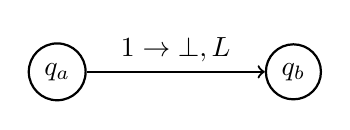
\begin{tikzpicture}
      % Draw circles
      \node[circle,draw,thick] (qa) at (0,0) {$q_a$};
      \node[circle,draw,thick] (qb) at (3,0) {$q_b$};
      
      % Connect circles with arrow
      \draw[->, thick] (qa) -- (qb) node[midway, above] {$1\to \bot,L$};
    \end{tikzpicture}
  \end{center}
  
  Since these windows are from two adjacent rows that represent taking the above transition, it cannot be the case, for example, that~$q_a$ appears in the bottom row of any of these windows.

  For simplicity, you can assume that the symbols in the cells of the window are restricted to $\set{0, 1, \bot,q_a,q_b}$.
  Recall that there can be other symbols in the rows, such as the ``boundary'' symbol~$\#$ and ``separator'' symbol $\$$, but we will ignore those here.
  
  To avoid having to write out many similar windows, you may use one or more variables~$s_i$ to indicate that a cell could have any of $0$, $1$, or~$\bot$.
  Such a variable, when repeated in multiple cells, represents the same symbol in every such cell.
  For example, instead of writing all three of the following windows (which may or may not be valid!):
  \[
    \begin{array}{|c|c|c|}
      \hline
      0 & 0 & 1 \\
      \hline
      0 & 0 & \bot \\
      \hline
    \end{array}
    \quad
    \begin{array}{|c|c|c|}
      \hline
      0 & 1 & 1 \\
      \hline
      1 & 0 & \bot \\
      \hline
    \end{array}
    \quad
    \begin{array}{|c|c|c|}
      \hline
      0 & \bot & 1 \\
      \hline
      \bot & 0 & \bot \\
      \hline
    \end{array}
  \]
  you could simply write
  \[\begin{array}{|c|c|c|}
      \hline
      0 & s_1 & 1 \\
      \hline
      s_1 & 0 & \bot \\
      \hline
    \end{array} \; .
  \]
  If needed, you may use multiple variables ($s_1, s_2, \ldots$) in a single window.

  Be sure to include all valid window contents that represent the head of the TM being in \emph{both} rows of the window, all those that represent the head being in \emph{only one} of the rows of the window, and all those that represent the head not being in the window at all.
  Do not include any invalid windows.

  You do not need to provide any justification. 

  \begin{solution}
  \begin{itemize}
  \item \textit{No head in either row:}
  \[
  \begin{array}{|c|c|c|}
  \hline
  s_1 & s_2 & s_3\\
  \hline
  s_1 & s_2 & s_3\\
  \hline
  \end{array}
  \]
  
  \item \textit{Head in the top row:}
  \[
  \begin{array}{|c|c|c|}
  \hline
  q_a & s_1 & s_2\\
  \hline
  \bot & s_1 & s_2\\
  \hline
  \end{array}
  \quad
  \begin{array}{|c|c|c|}
  \hline
  s_1 & q_a & s_2\\
  \hline
  q_b & \bot & s_2\\
  \hline
  \end{array}
  \quad
  \begin{array}{|c|c|c|}
  \hline
  s_1 & s_2 & q_a\\
  \hline
  s_1 & q_b & \bot\\
  \hline
  \end{array}
  \]
  
  \item \textit{Head in the bottom row:}
  \[
  \begin{array}{|c|c|c|}
  \hline
  s_1 & s_2 & s_3 \\
  \hline
  q_b & s_2 & s_3 \\
  \hline
  \end{array}
  \quad
  \begin{array}{|c|c|c|}
  \hline
  s_1 & s_2 & s_3 \\
  \hline
  s_1 & q_b & s_3 \\
  \hline
  \end{array}
  \quad
  \begin{array}{|c|c|c|}
  \hline
  s_1 & s_2 & s_3 \\
  \hline
  s_1 & s_2 & q_b \\
  \hline
  \end{array}
  \]
  
  \item \textit{Head in both rows:}
  \[
  \begin{array}{|c|c|c|}
  \hline
  s_1 & s_2 & q_a\\
  \hline
  s_1 & q_b & \bot\\
  \hline
  \end{array}
  \quad
  \]
  \end{itemize}
  \end{solution}

   \part [5] In the proof of Cook-Levin Theorem, we claimed that:
   \begin{quote}
        If every 2-by-3 window is valid, and the first row is the start configuration, then each row of the tableau is a configuration that yields the next row.
   \end{quote}

    Interestingly, the claim does not hold for 2-by-2 windows: it is possible for all $2 \times 2$ windows to be valid while the overall transition is invalid. 

    Give an example by first defining one or more Turing machine transitions, then providing two adjacent rows where each $2 \times 2$ window is valid, but the transition is incorrect. 

    \hint{consider an invalid pair of rows in which the active state of the head ``disappears''.}

    \label{CL-window-b}

    \begin{solution}
    Define a Turing machine with a transition 
    \[
    \delta(q_c,\,1)=(q_c,\,1,\,R).
    \]
    Consider these two adjacent rows of length 3:
    
    \[
    \text{Top row: } \quad q_c \quad 1 \quad 1 
    \]
    \[
    \text{Bottom row: } \quad 1 \quad 1 \quad 1
    \]
    
    Every $2\times 2$ window in these rows is locally valid as no symbols conflict with the machine's rules. However, the machine's state $q_c$ disappears incorrectly from the second row, making the overall transition invalid.
    \end{solution}

    \part [4] Towards proving the Cook-Levin Theorem in lecture, we outlined a proof of the following statement: 
    \begin{quote}
      Let language $L \in \NP$ be arbitrary, and fix an efficient verifier $\textsc{VerifyL}$ for~$L$.
      Given any instance $x$ of $L$, in polynomial time we can construct an instance $\phi$ of $\SAT$ such that $\phi$ is satisfiable \emph{if and only if} there \emph{exists} a $c$ such that the tableau of $\textsc{VerifyL}(x,c)$ has $q_\text{accept}$ in it.
    \end{quote}
    Briefly explain why proving this statement proves that SAT is \NP-hard.
    
    \begin{solution}
    Proving that the constructed $\phi$ is satisfiable if and only if there exists a $c$ with $q_{\text{accept}}$ in the tableau of $\textsc{VerifyL}(x,c)$ establishes a PTMR from every language in \NP{} to $\SAT$, showing that $\SAT$ is \NP-hard.
    \end{solution}

    \end{parts}
  
\end{questions}

\end{document}
